\section{Arquitectura de Software}

El desarrollo de Navindoor se ha dividido en módulos claramente diferenciados, que siguen los pasos para el posicionamiento mencionado en la introducción. A continuación describiremos cada una de ellas.


% ----------------------------------------------------------------------



\subsection{Planimetría}


Para la definición del escenario se ha definido clases en MATLAB que representarán los distitnos objetos necesarios para crear una planimetría.  Ya que en un principo las trajectorias se definen en un edificio, la clase más grande que contiene los demás elementos, es la clase \emph{building} (figura \ref{fig:esquemabuilding}). Estos objetos pueden contener objetos \emph{level} que representa las plantas. A su vez, los objetos \emph{level}, contienen objetos \emph{walls}, \emph{doors}, \emph{beacons}, \emph{stairs} y \emph{elevators}.  Todos estos objetos contiene la posición y otras relaciones entre ellos para definir completamente la planimetría. 


\begin{figure}[!ht]
    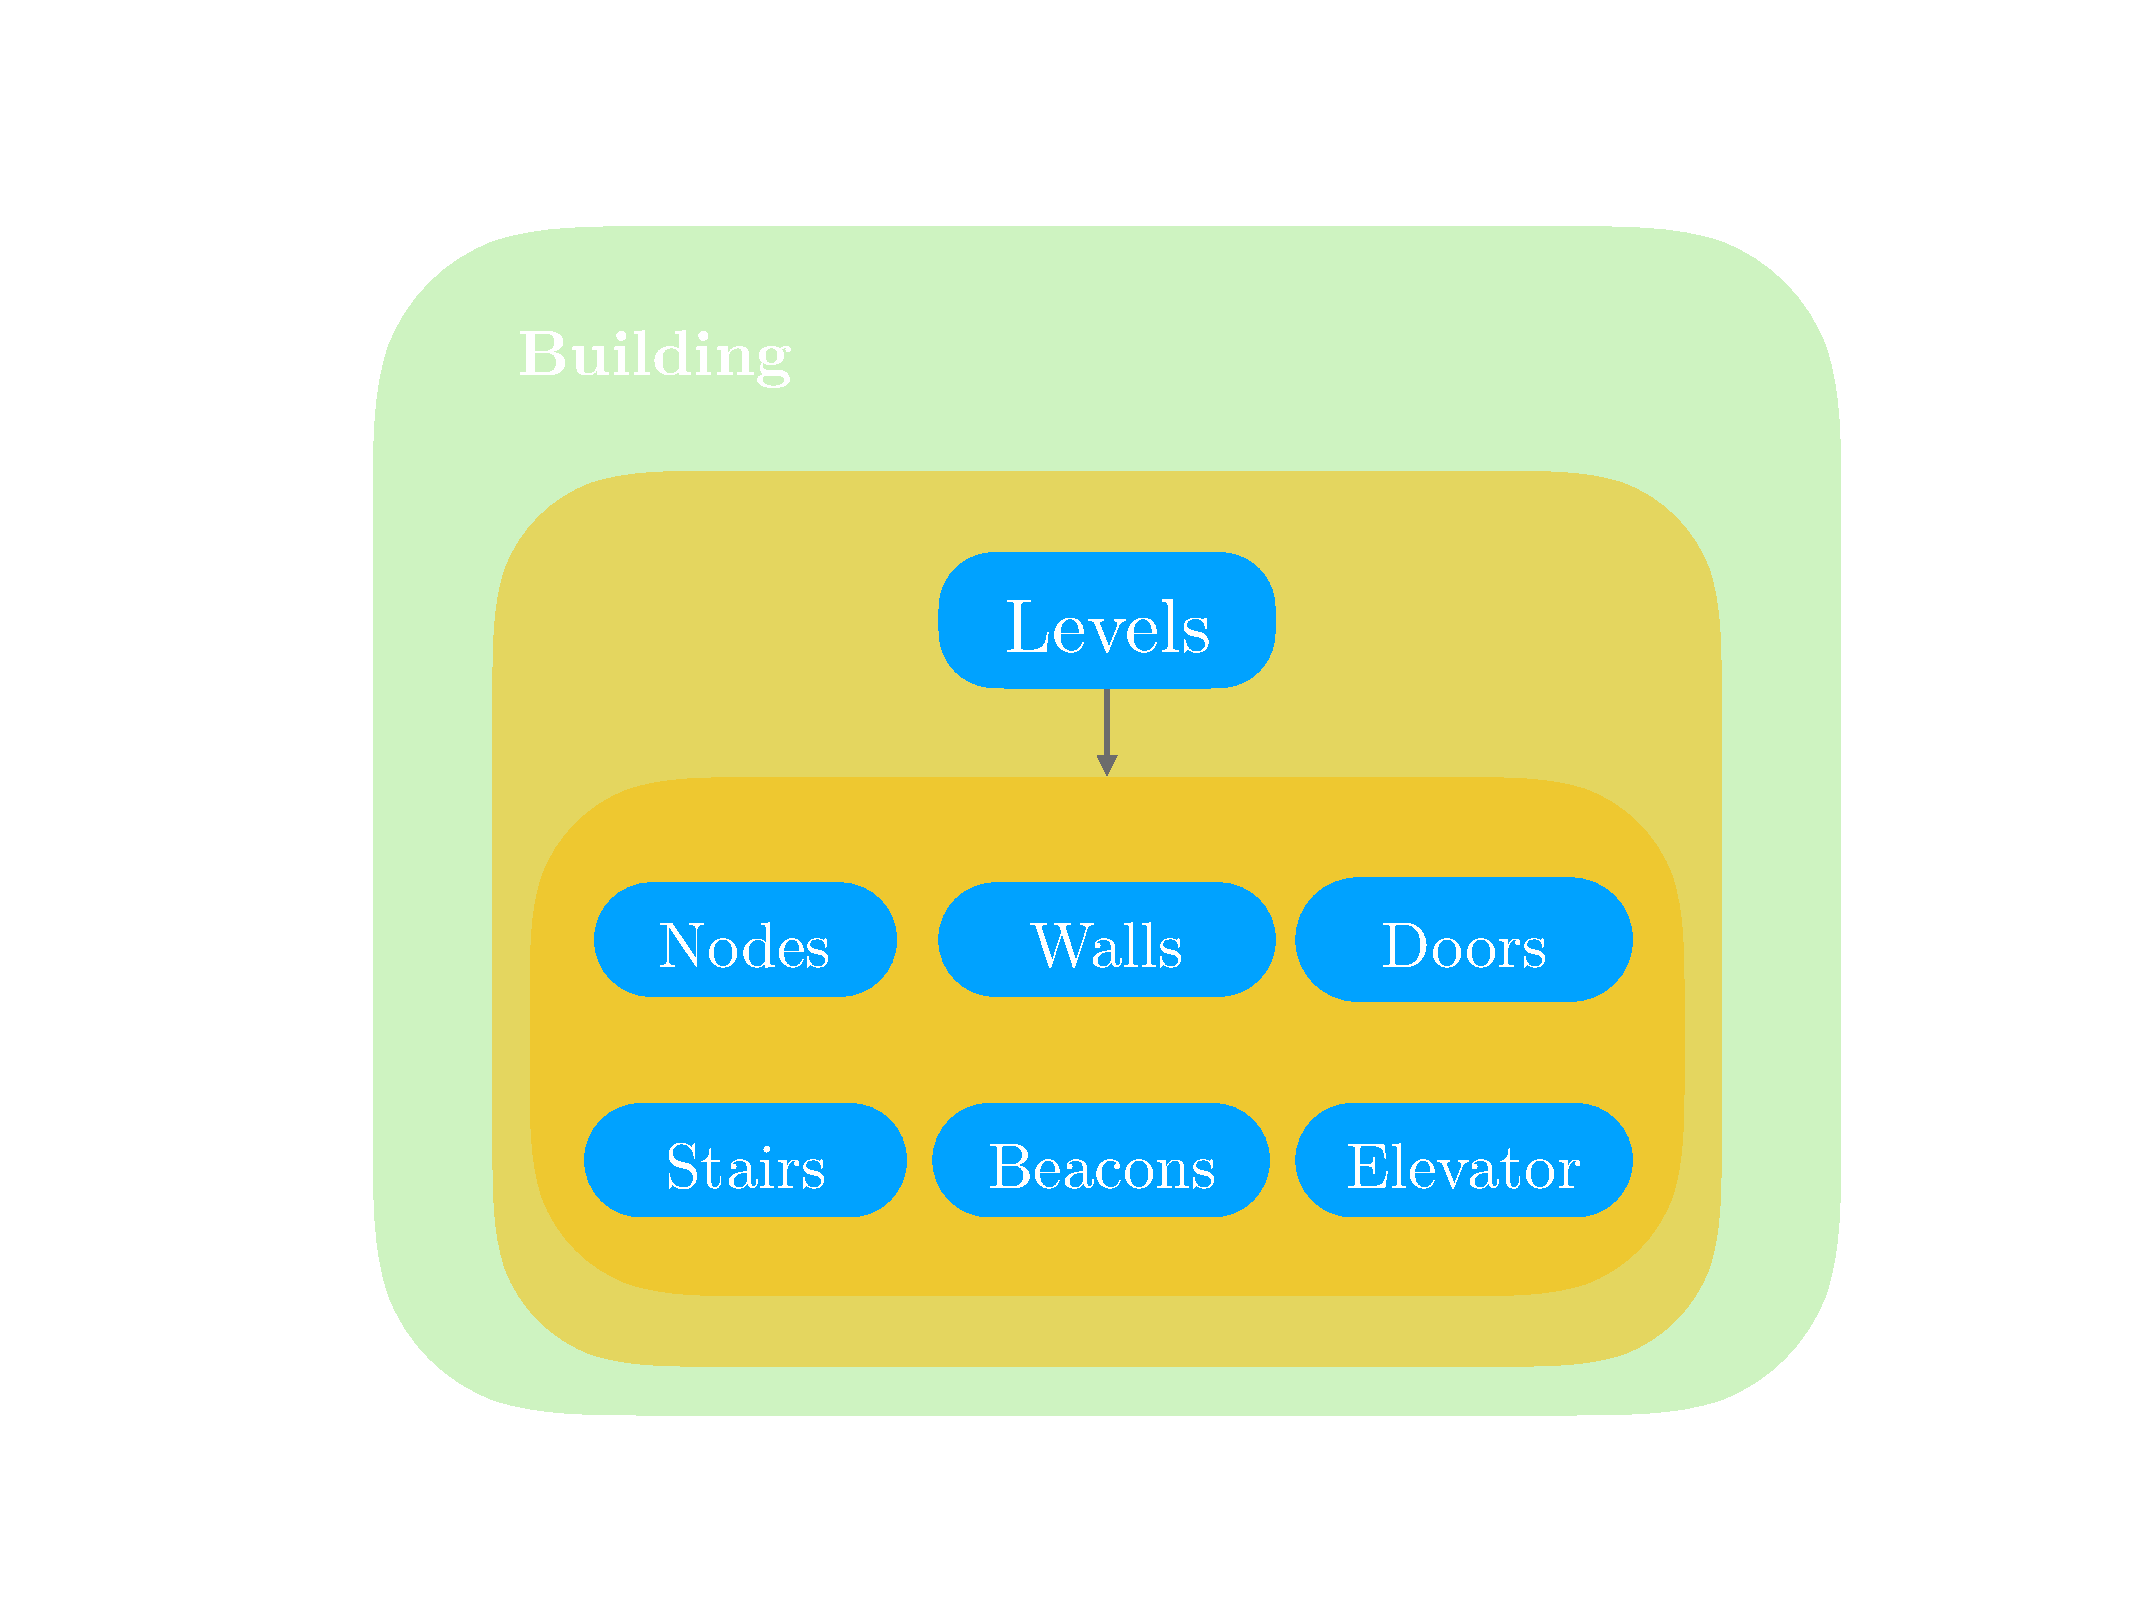
\includegraphics[width=1.0\columnwidth]{img/Design/1.pdf}
    \caption[]{Esquema de la clase \emph{building}}
    \label{fig:esquemabuilding}
\end{figure}

Con estos objeto podemos determinar que trajectorias son posibles en un objeto \emph{building}, asi como el tipo de camino esta siguiendo el peatón, (muy util a la hora de simular la trayectoria), además de definir la distribución de los \emph{beacons}. 

\begin{figure}[!ht]
    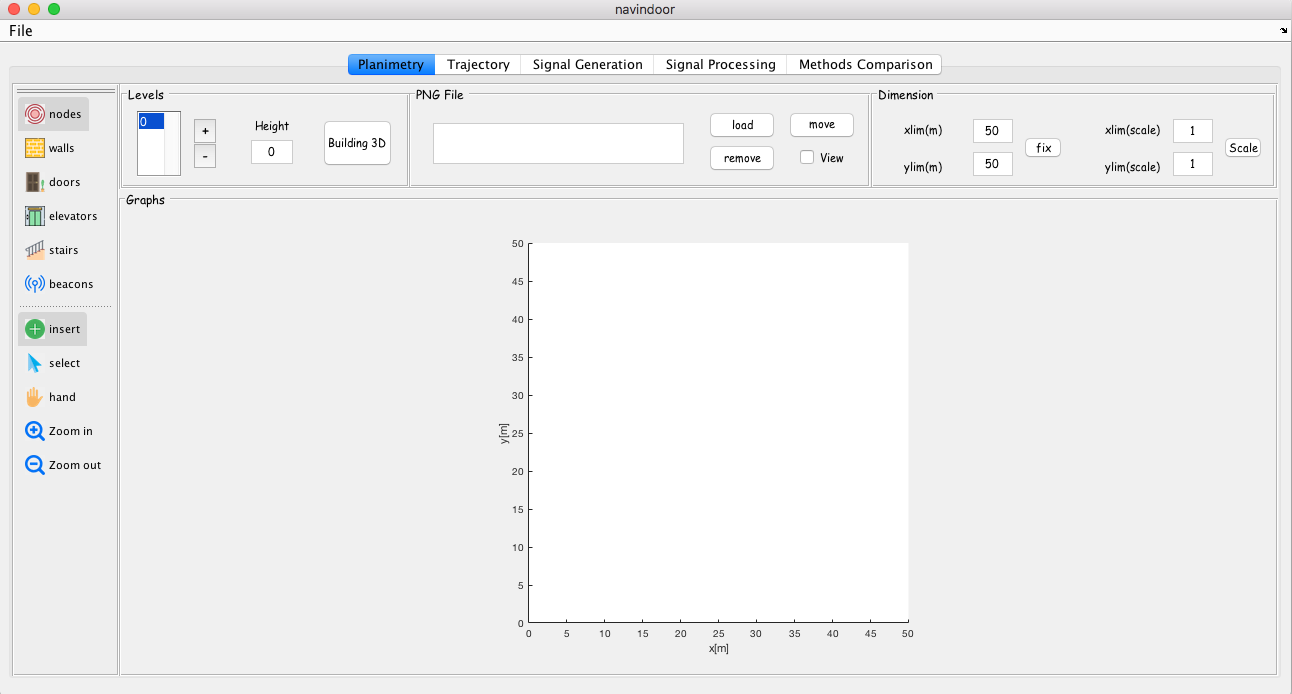
\includegraphics[width=1.0\columnwidth]{img/Design/1-interfaz.png}
    \caption[]{Interfaz gráfica para el diseño de la planimetría \emph{building}}
    \label{fig:interfaz1}
\end{figure}

Debido a que el proceso de creación de la planimteria, Navindoor contiene una interfaz gráfica  capaz de generar un objeto \emph{building} (figura \ref{fig:interfaz1}).  De esta forma podemos cargar nuestras imagenes de la planimtería de interés, y guardarlo en un archivo tipo \emph{.mat}, que luego puede ser utilizada por la propia interfaz o por en la propia consola de MATLAB. 



Debemos notar que la clase building es una abstración de la planimetría de un edificio, por lo que la traslacíon a otros formatos como \emph{XML} o \emph{JSON} son posible, y ya se estan explorando por parte del equipo de desarrollo. Este desarrollo permitirá comunicaciones con plataformas como \emph{Open Street Maps}.


% ----------------------------------------------------------------------


\subsection{Trayectorias}
\begin{figure}
    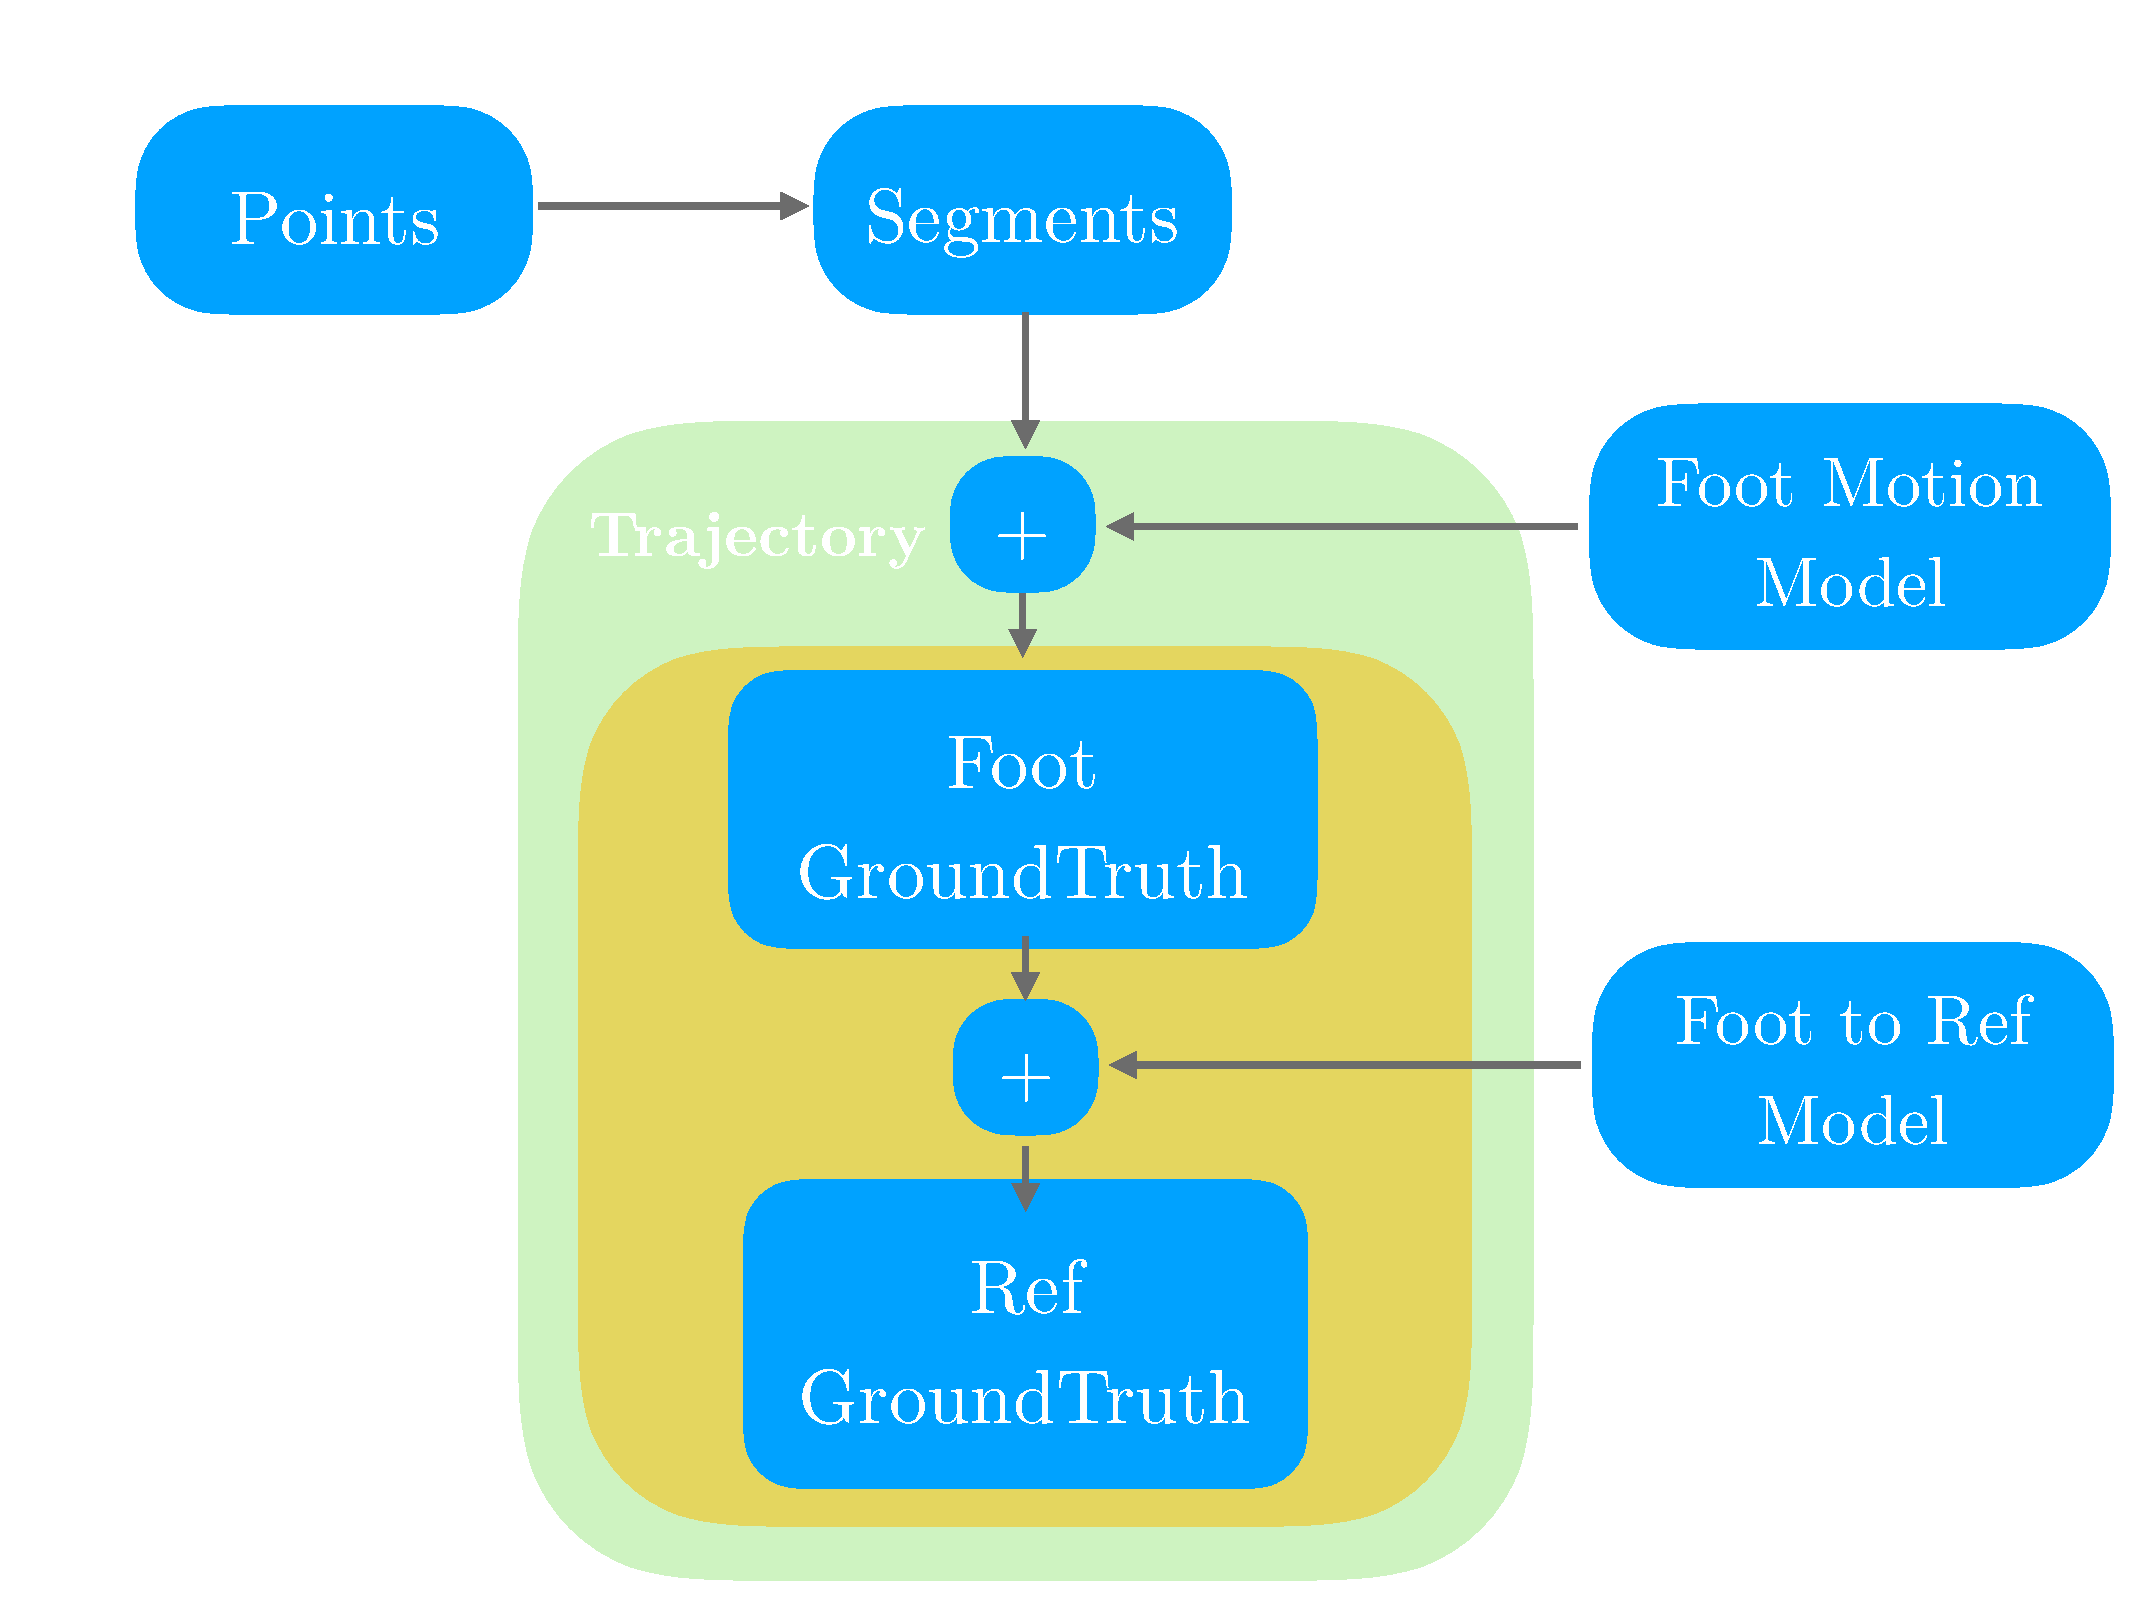
\includegraphics[width=1.0\columnwidth]{img/Design/2.pdf}
    \caption[]{Visualización de la Facultad de ingeniería}
\end{figure}
% ----------------------------------------------------------------------
\subsection{Señales}
Para la representación de las  señales se ha creado un objeto MATLAB ...
\begin{figure}
    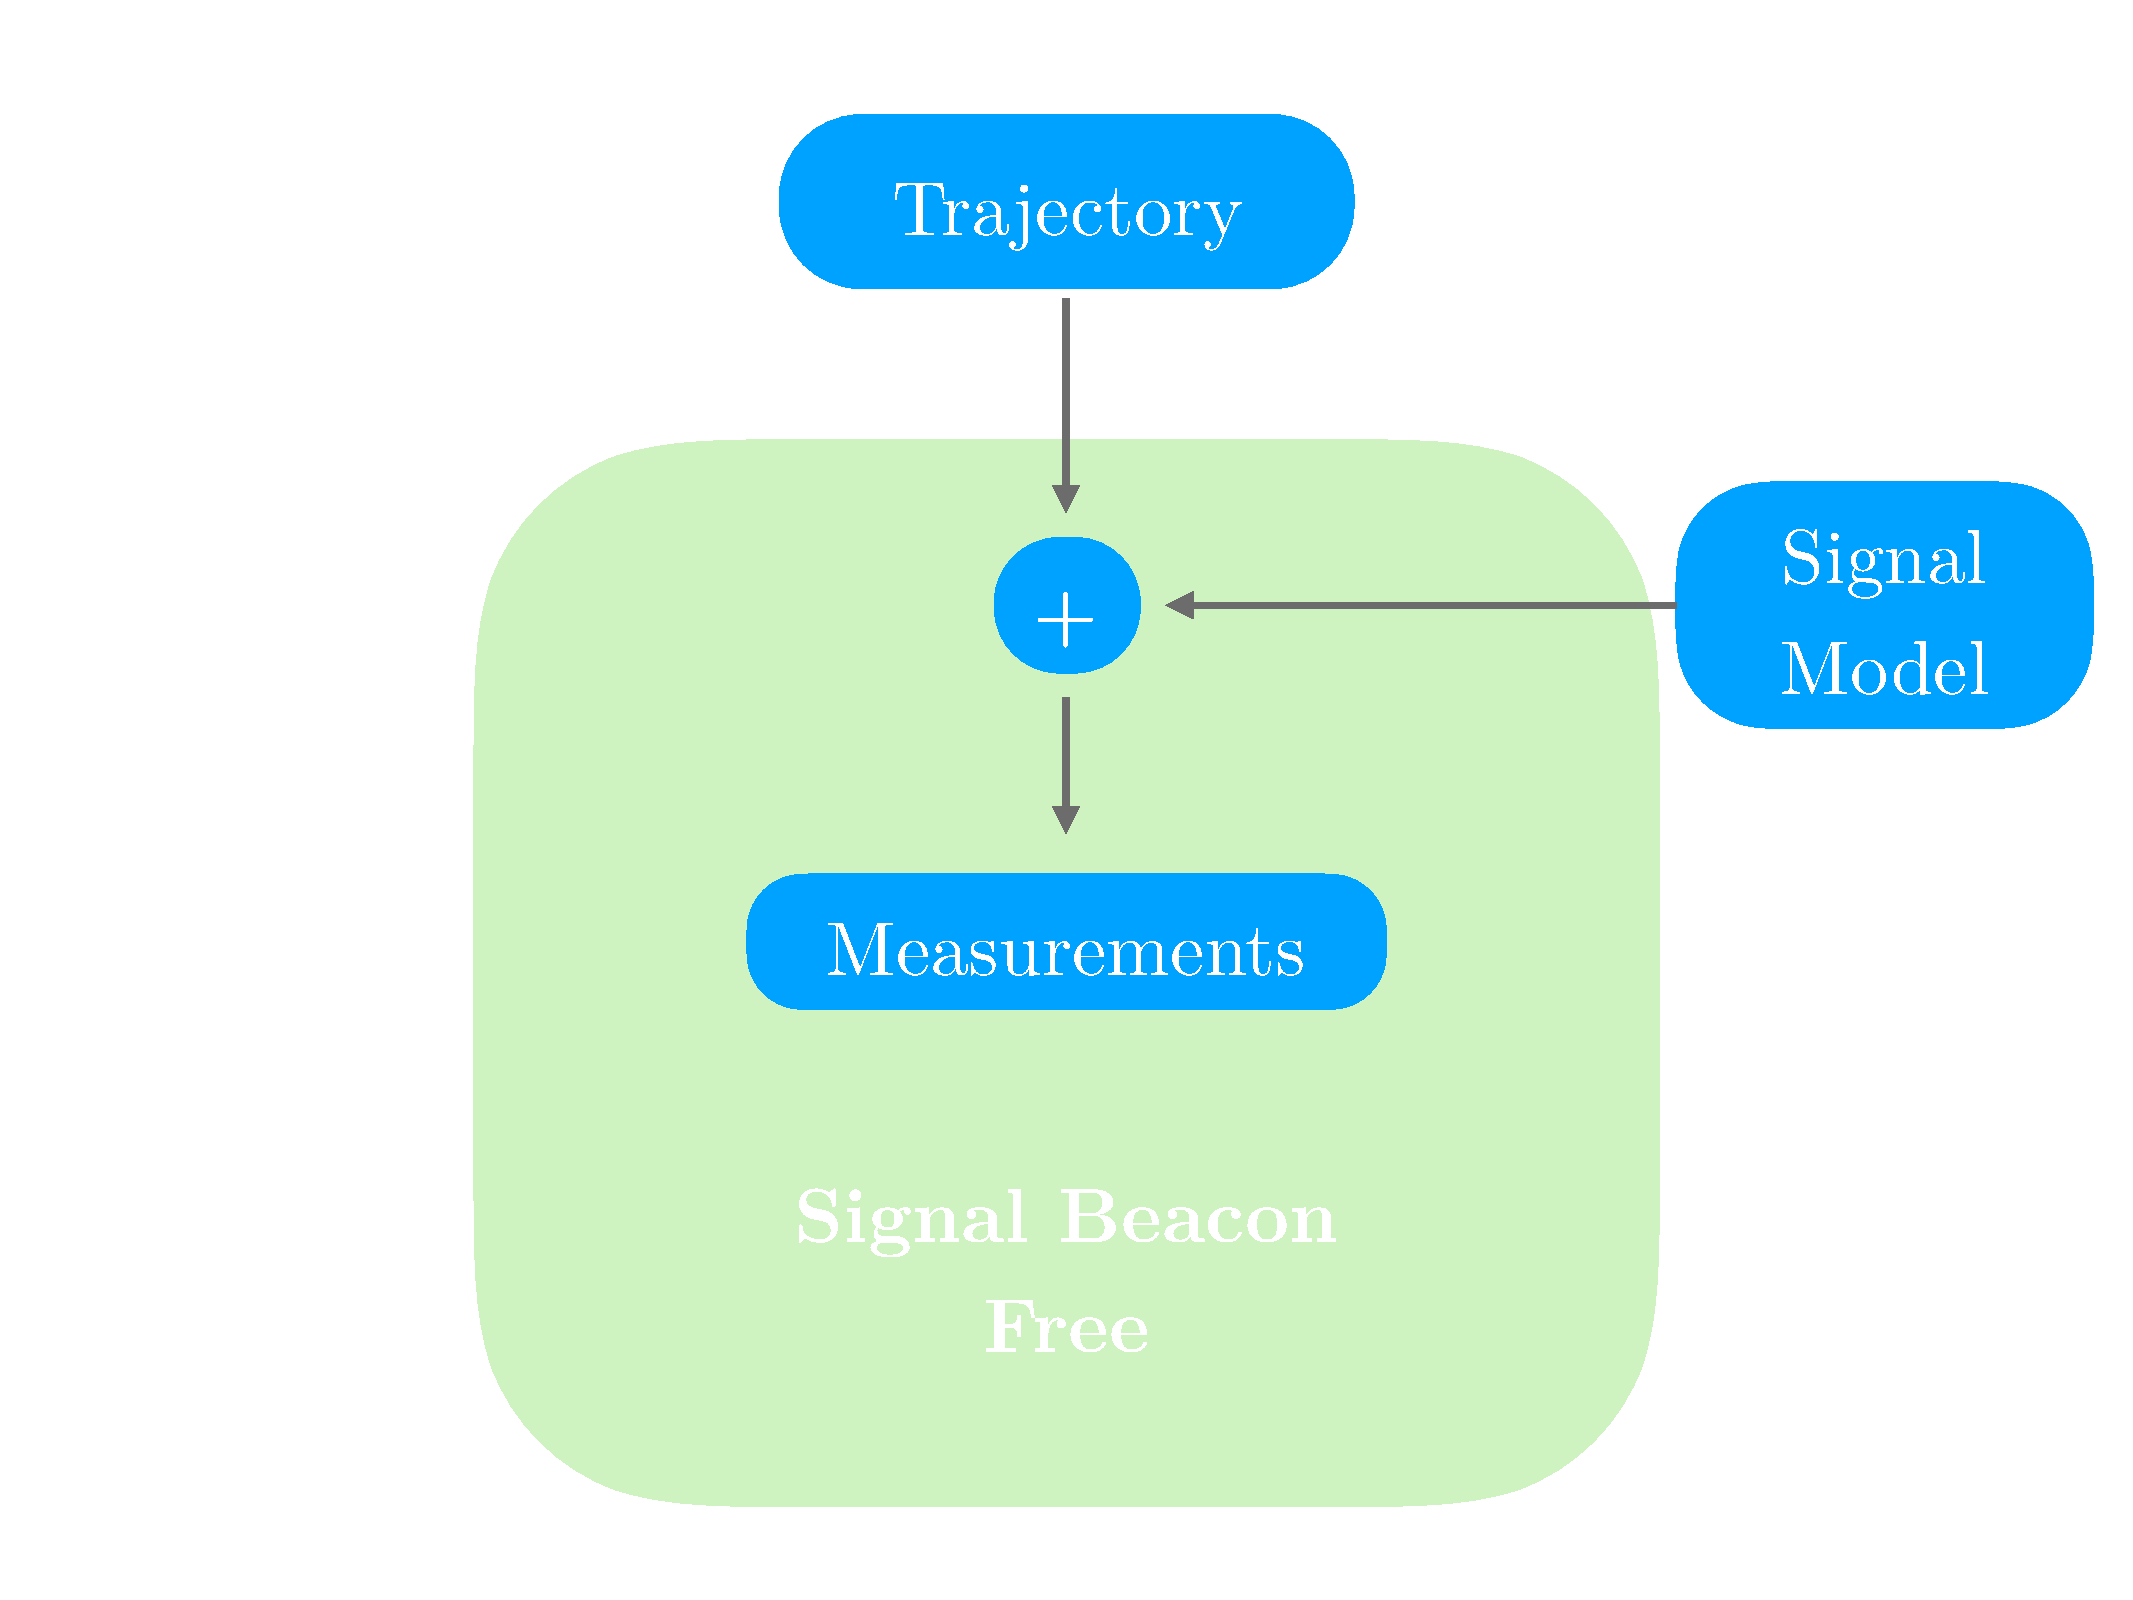
\includegraphics[width=1.0\columnwidth]{img/Design/3.pdf}
    \caption[]{Visualización de la Facultad de ingeniería}
\end{figure}
\begin{figure}
    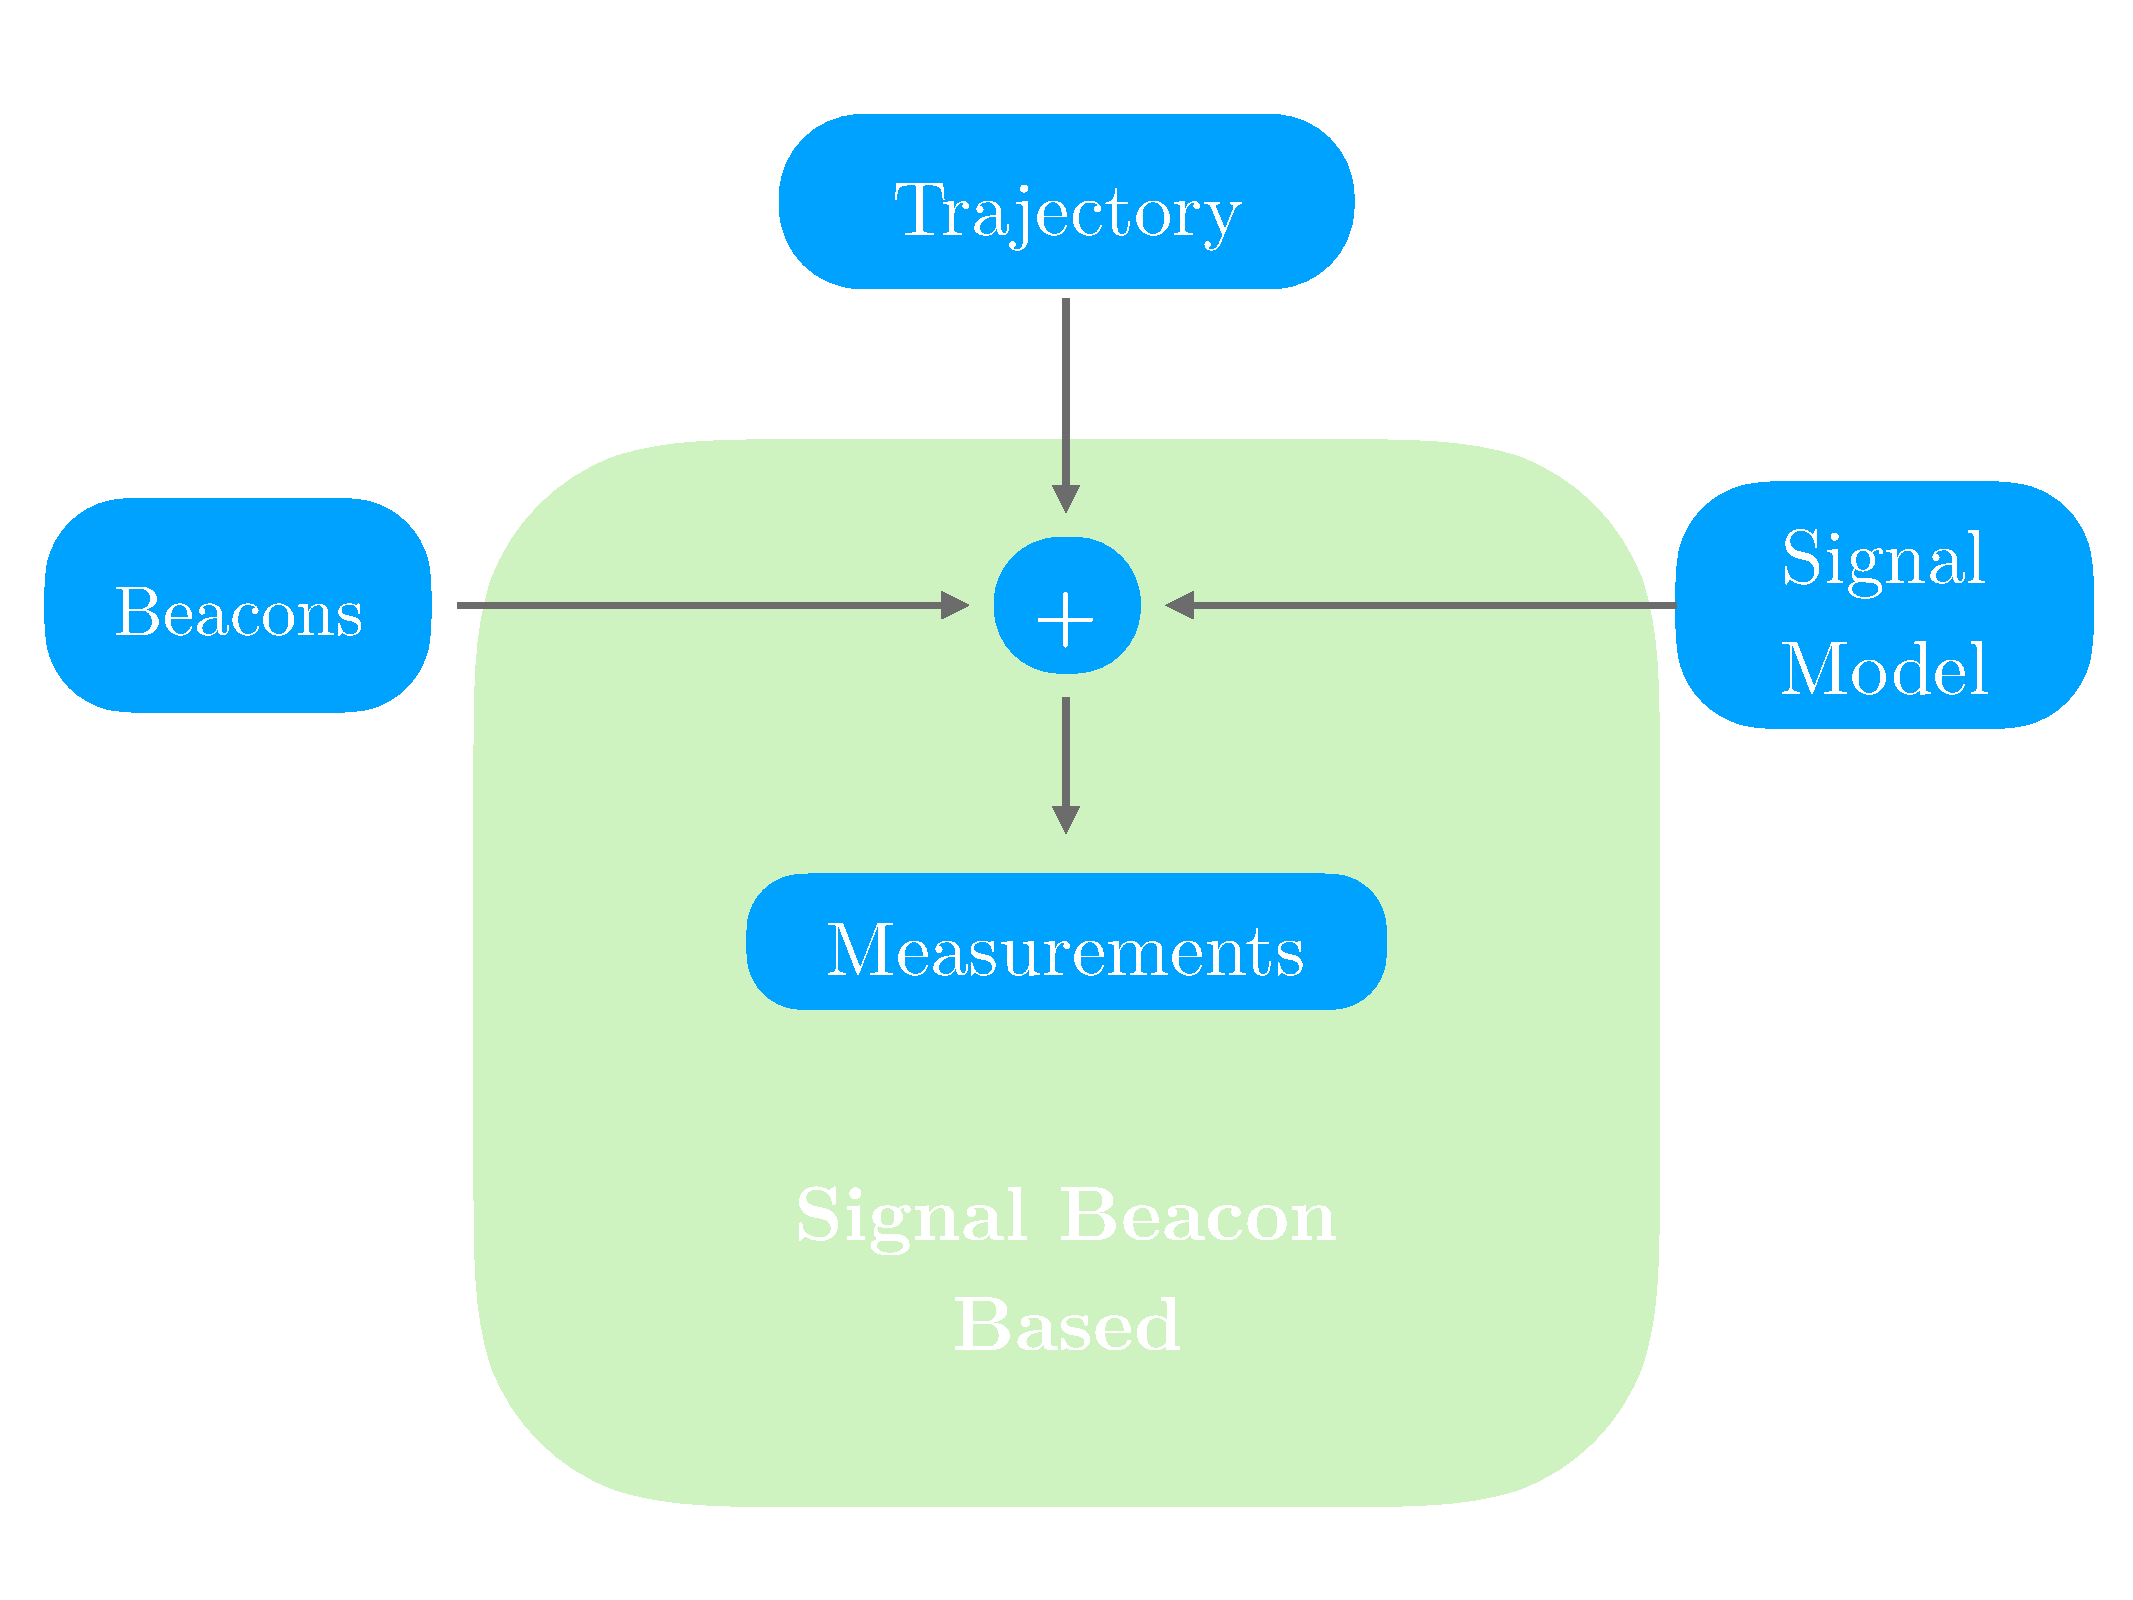
\includegraphics[width=1.0\columnwidth]{img/Design/4.pdf}
    \caption[]{Visualización de la Facultad de ingeniería}
\end{figure}
% ----------------------------------------------------------------------
\subsection{Procesamiento}
\begin{figure}
    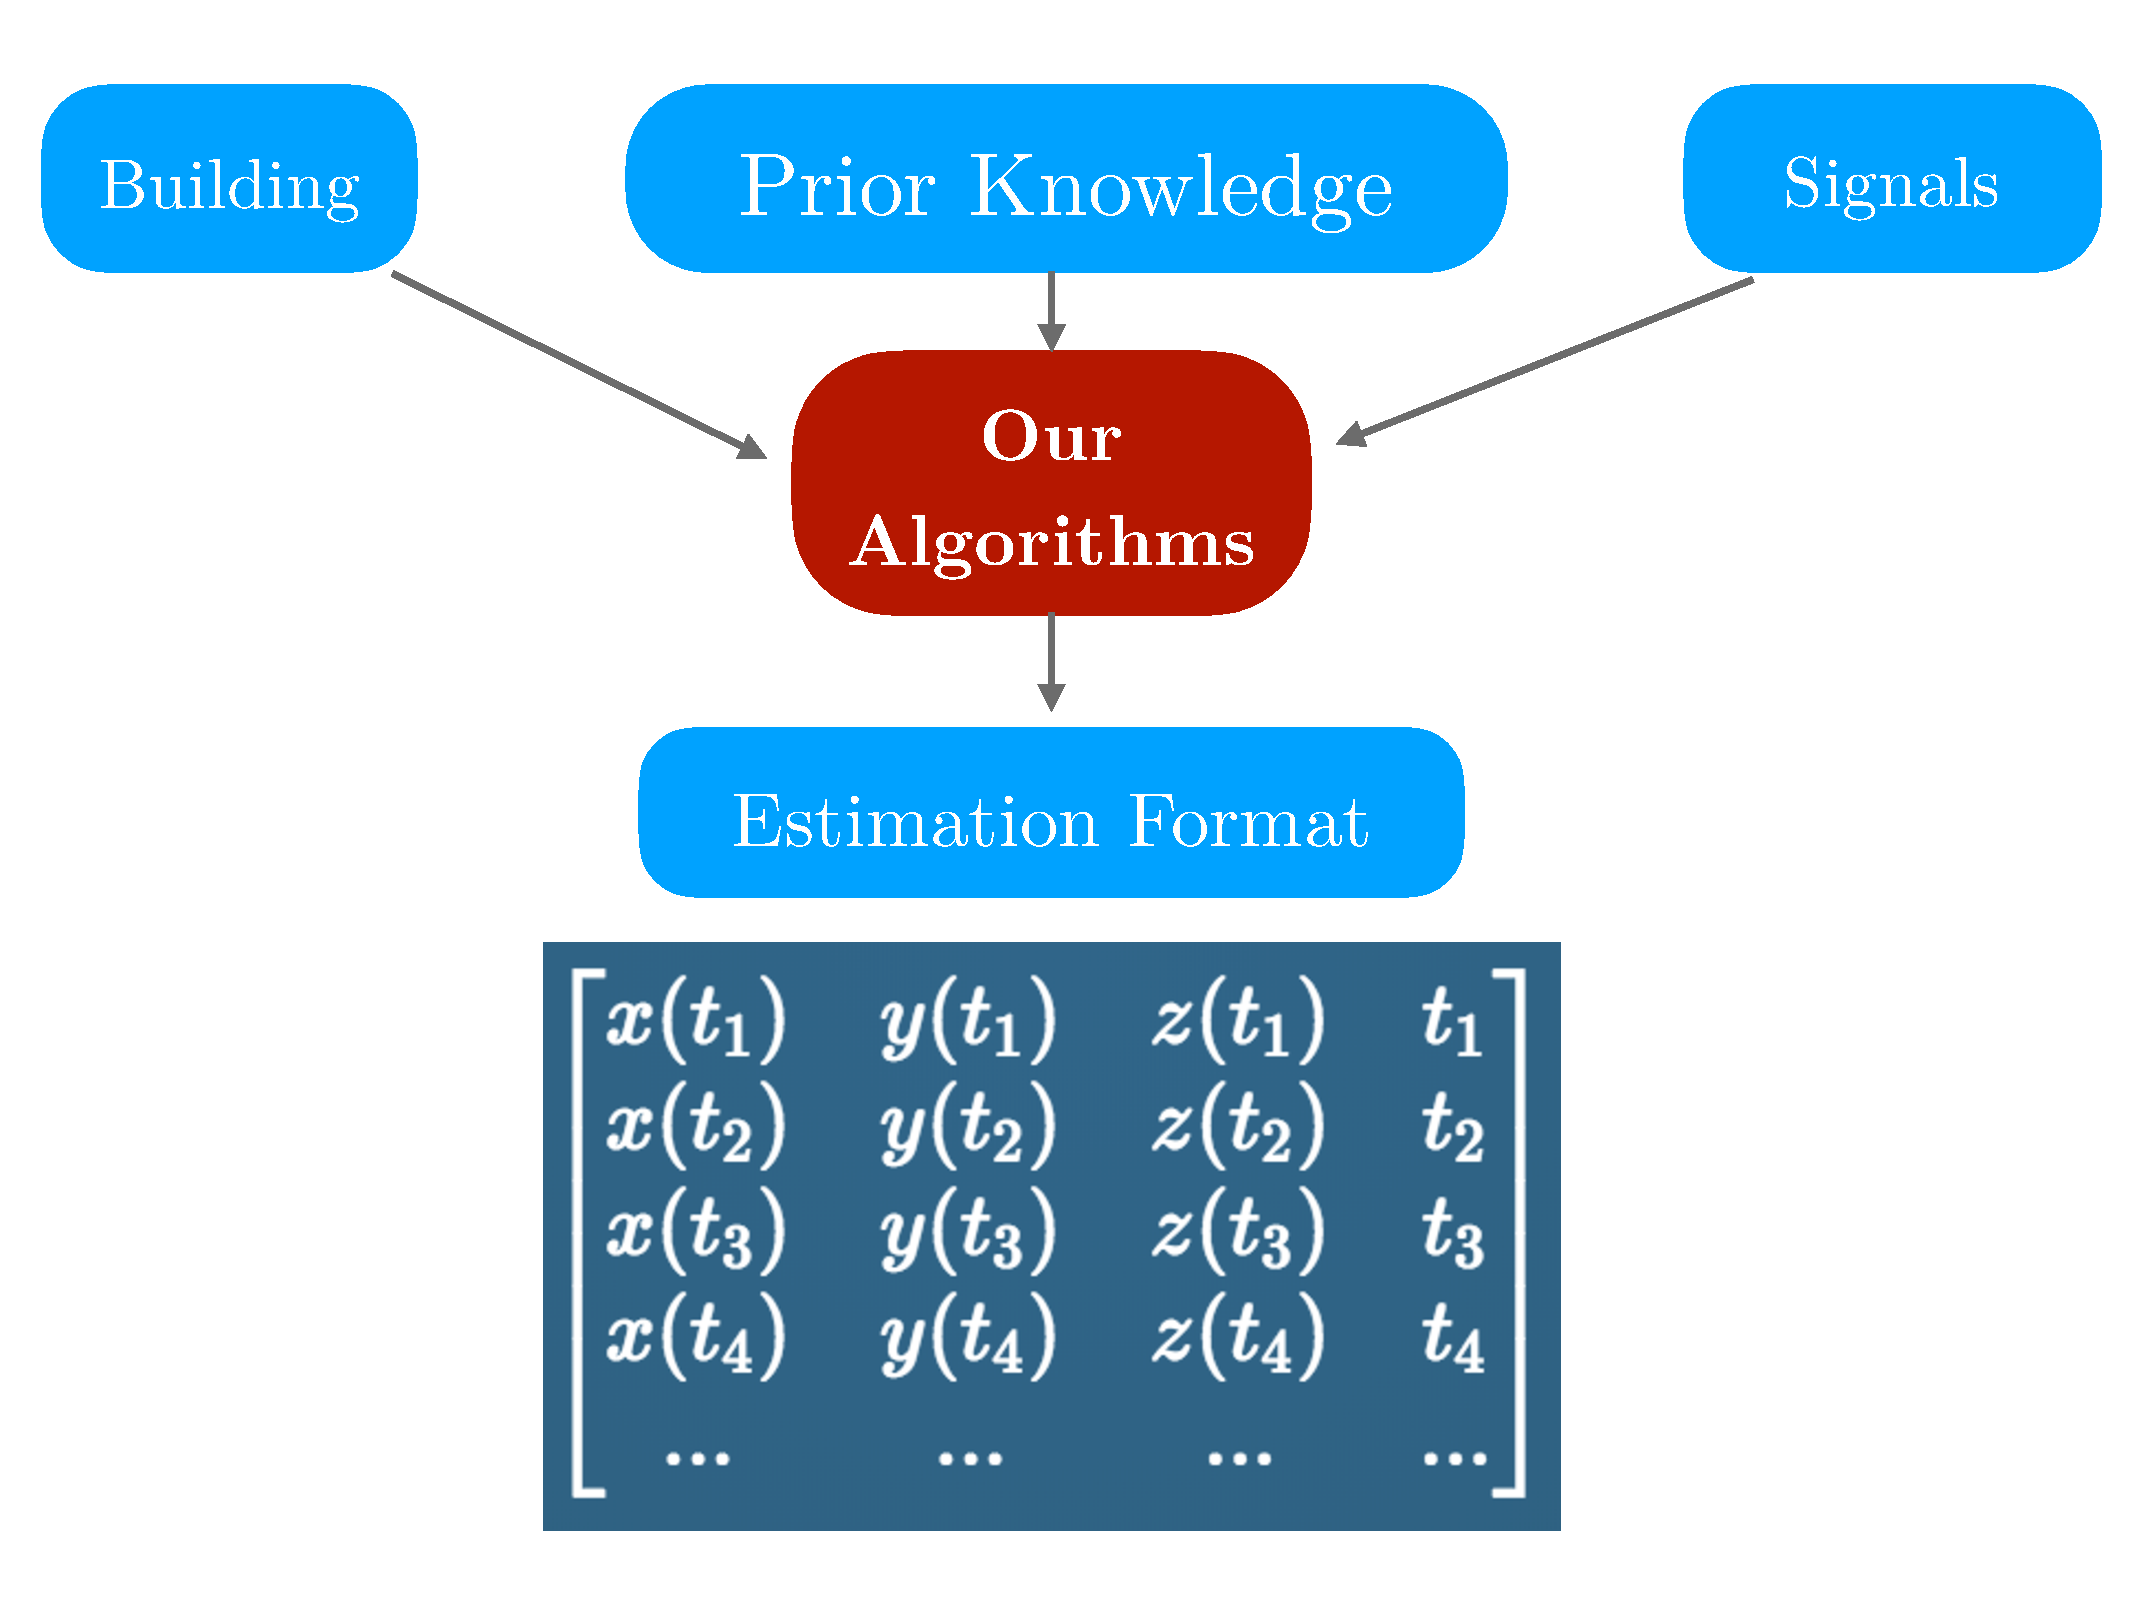
\includegraphics[width=1.0\columnwidth]{img/Design/5.pdf}
    \caption[]{Visualización de la Facultad de ingeniería}
\end{figure}
% ----------------------------------------------------------------------
\subsection{Comparación}